%% %%%%%%%%%%%%%%%%%%%%%%%%%%%%%%%%%%%%%%%%%%%%%%%%%
%% Work of Baeza Olvera Daniel Jesus, making use of this template, all credits due to the original creaters below:
%% Template for a conference paper, prepared for the
%% Food and Resource Economics Department - IFAS
%% UNIVERSITY OF FLORIDA
%% %%%%%%%%%%%%%%%%%%%%%%%%%%%%%%%%%%%%%%%%%%%%%%%%%
%% Version 1.0 // November 2019
%% %%%%%%%%%%%%%%%%%%%%%%%%%%%%%%%%%%%%%%%%%%%%%%%%%
%% Ariel Soto-Caro
%%  - asotocaro@ufl.edu
%%  - arielsotocaro@gmail.com
%% %%%%%%%%%%%%%%%%%%%%%%%%%%%%%%%%%%%%%%%%%%%%%%%%%
\documentclass[11pt]{article}
\usepackage{UF_FRED_paper_style}
\usepackage{lipsum}  %% Package to create dummy text (comment or erase before start)


%% ===============================================
%% Setting the line spacing (3 options: only pick one)
% \doublespacing
% \singlespacing
\onehalfspacing
%% ===============================================

\setlength{\droptitle}{-5em} %% Don't touch

% %%%%%%%%%%%%%%%%%%%%%%%%%%%%%%%%%%%%%%%%%%%%%%%%%%%%%%%%%%
% SET THE TITLE
% %%%%%%%%%%%%%%%%%%%%%%%%%%%%%%%%%%%%%%%%%%%%%%%%%%%%%%%%%%

% TITLE:
\title{Applied Data Science Capstone: The Battle of Neighborhoods
\thanks{Presentation for the Capstone project, part of Applied Data Science Specialization, Coursera.}
}

% AUTHORS:
\author{Baeza Olvera Daniel Jesus\\% Name author
    \href{mailto:daniil_iisus@icloud.com}{\texttt{daniil_iisus@icloud.com}} %% Email author 1 
%\and Forth Author\\% Name author
%    \href{mailto:forthuthor@ufl.edu}{\texttt{forthuthor@ufl.edu}}%% Email author 4
    }
    
% DATE:
\date{\today}

% %%%%%%%%%%%%%%%%%%%%%%%%%%%%%%%%%%%%%%%%%%%%%%%%%%%%%%%%%%
% %%%%%%%%%%%%%%%%%%%%%%%%%%%%%%%%%%%%%%%%%%%%%%%%%%%%%%%%%%
\begin{document}
% %%%%%%%%%%%%%%%%%%%%%%%%%%%%%%%%%%%%%%%%%%%%%%%%%%%%%%%%%%
% %%%%%%%%%%%%%%%%%%%%%%%%%%%%%%%%%%%%%%%%%%%%%%%%%%%%%%%%%%
% ABSTRACT
% %%%%%%%%%%%%%%%%%%%%%%%%%%%%%%%%%%%%%%%%%%%%%%%%%%%%%%%%%%
% %%%%%%%%%%%%%%%%%%%%%%%%%%%%%%%%%%%%%%%%%%%%%%%%%%%%%%%%%%
{\setstretch{.8}

% %%%%%%%%%%%%%%%%%%
\begin{abstract}
% CONTENT OF ABS HERE--------------------------------------
As part of the IBM \& Coursera Applied Data Science Specialization, it is required to do a small research using the taught data science methodologies and data sources.
The data science methodologies and data sources that had more emphasis were, Geographical Data with the Python package Folium, and the usage of third party APIs for retrieval of location data.
\newline

The problem that this little research tackles is about Food Venues, especially Mexican Food venues in the city of Naha, Okinawa Japan which is the place I wish to live in the not so distant future. One of my plans while living there is Co-owning a Mexican Food restaurant.
% END CONTENT ABS------------------------------------------
\newline

\noindent
\textit{\textbf{Keywords: }%
Data Science; Foursquare; GIS; Google Maps API; Capstone, Python.} \\ %% <-- Keywords HERE!
\end{abstract}
}

% %%%%%%%%%%%%%%%%%%%%%%%%%%%%%%%%%%%%%%%%%%%%%%%%%%%%%%%%%%
% %%%%%%%%%%%%%%%%%%%%%%%%%%%%%%%%%%%%%%%%%%%%%%%%%%%%%%%%%%
% BODY OF THE DOCUMENT
% %%%%%%%%%%%%%%%%%%%%%%%%%%%%%%%%%%%%%%%%%%%%%%%%%%%%%%%%%%
% %%%%%%%%%%%%%%%%%%%%%%%%%%%%%%%%%%%%%%%%%%%%%%%%%%%%%%%%%%

% --------------------
\section{Introduction}
% --------------------

In this project we will try to find an optimal location for a restaurant.
\newline

Specifically, this report will be targeted to stakeholders (mainly Myself) interested in opening a Mexican Taqueria in Naha City, Okinawa, Japan. The focus of this is looking for locations that are not already crowded with restaurants. We are also particularly interested in areas with no Mexican restaurants in vicinity. We would also prefer locations as close to the IT COLLEGE as possible, this because IT people love tacos and because I'd love to work as a teacher there and have tacos after class, but only assuming that first two conditions are met. We will use a data science approach to select the most promissing neighborhoods based on this criteria. Advantages of each area will then be clearly expressed so that taking a decision using the top neighborhoods will be simplyfied.
\newline

All of this is part of the final project for the Applied Data Science Specialization offered by IBM Through Coursera.

\cite{course} % Example of citation. Erase before use

% --------------------
\section{Data}
% --------------------

Based on definition of our problem, factors that will influence our decission are:
\begin{itemize}
    \item Number of existing restaurants in the neighborhood (any type of restaurant)
    \item Number of and distance to Mexican restaurants in the neighborhood, if any
    \item Distance of neighborhood from IT College
\end{itemize}

Following the project example, I decided to also use regularly spaced grid of locations, centered around city center, to define our neighborhoods. In fact I will mostly use the same approach and step by step analysis, due to time constraint and not having any other particulary interesting problem to solve using the foursquare API which is required for this project.

\cite{courseNotebook} % Example of citation. Erase before use
\newline

Following data sources will be needed to extract/generate the required information:
\begin{itemize}
    \item Centers of candidate areas will be generated algorithmically and approximate addresses of centers of those areas will be obtained using Google Maps API reverse geocoding.
    \item Number of restaurants and their type and location in every neighborhood will be obtained using Foursquare API.
    \item Coordinates of the IT college will be obtained using Google Maps API geocoding.
\end{itemize}

\noindent
\cite{foursquare}
\newline
\cite{googleApi}

\subsection{Neighborhood Candidates}

Let's create latitude \& longitude coordinates for centroids of our candidate neighborhoods. We will create a grid of cells covering our area of interest which is aprox. 6x6 killometers centered around Naha city center.
\newline
Let's first find the latitude \& longitude of IT College, using specific, well known address and Google Maps geocoding API.
\newline
Now let's create a grid of area candidates, equaly spaced, centered around city center and within ~3km from IT College. Our neighborhoods will be defined as circular areas with a radius of 300 meters, so our neighborhood centers will be 600 meters apart.
\newline
To accurately calculate distances we need to create our grid of locations in Cartesian 2D coordinate system which allows us to calculate distances in meters (not in latitude/longitude degrees). Then we'll project those coordinates back to latitude/longitude degrees to be shown on Folium map. So let's create functions to convert between WGS84 spherical coordinate system (latitude/longitude degrees) and UTM Cartesian coordinate system (X/Y coordinates in meters).
\newline

\begin{figure}[H]
    \centering
        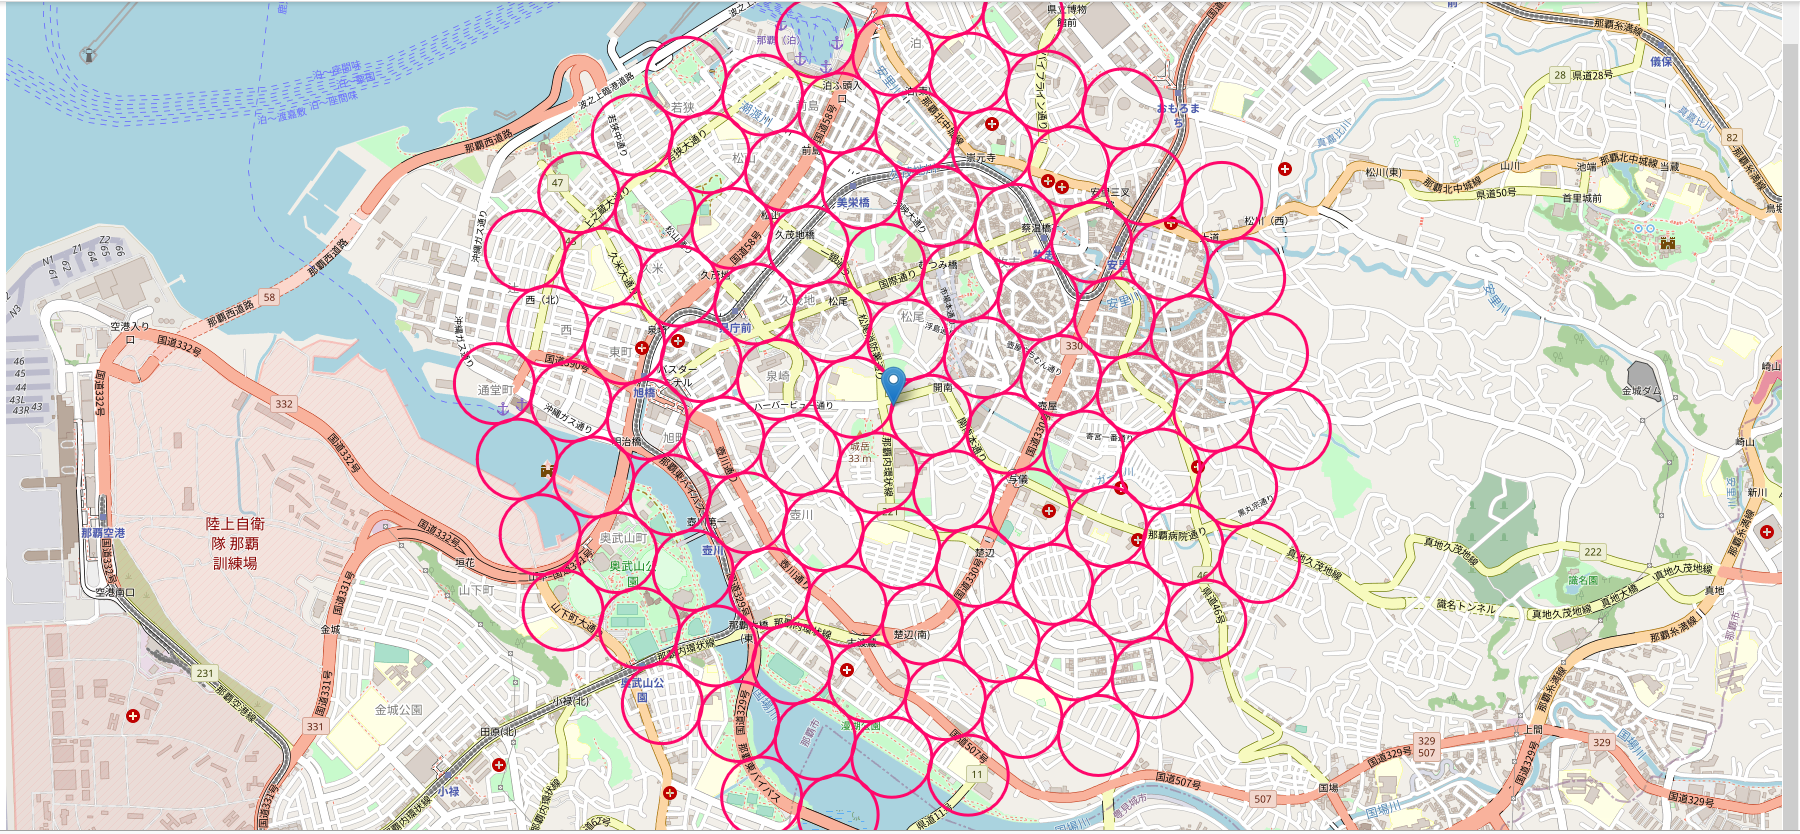
\includegraphics[scale=.3]{figures/cm1.png}
    \caption{Candidate Locations.}
    \label{fig:1}
\end{figure}

Now that we have our location candidates, let's use Foursquare API to get info on restaurants in each neighborhood.
\newline
We're interested in venues in 'food' category, but only those that are proper restaurants - coffe shops, pizza places, bakeries etc. are not direct competitors so we don't care about those. So we will include in out list only venues that have 'restaurant' in category name, and we'll make sure to detect and include all the subcategories of specific 'Mexican restaurant' category, as we need info on Mexican restaurants in the neighborhood.
\newline

\begin{figure}[H]
    \centering
        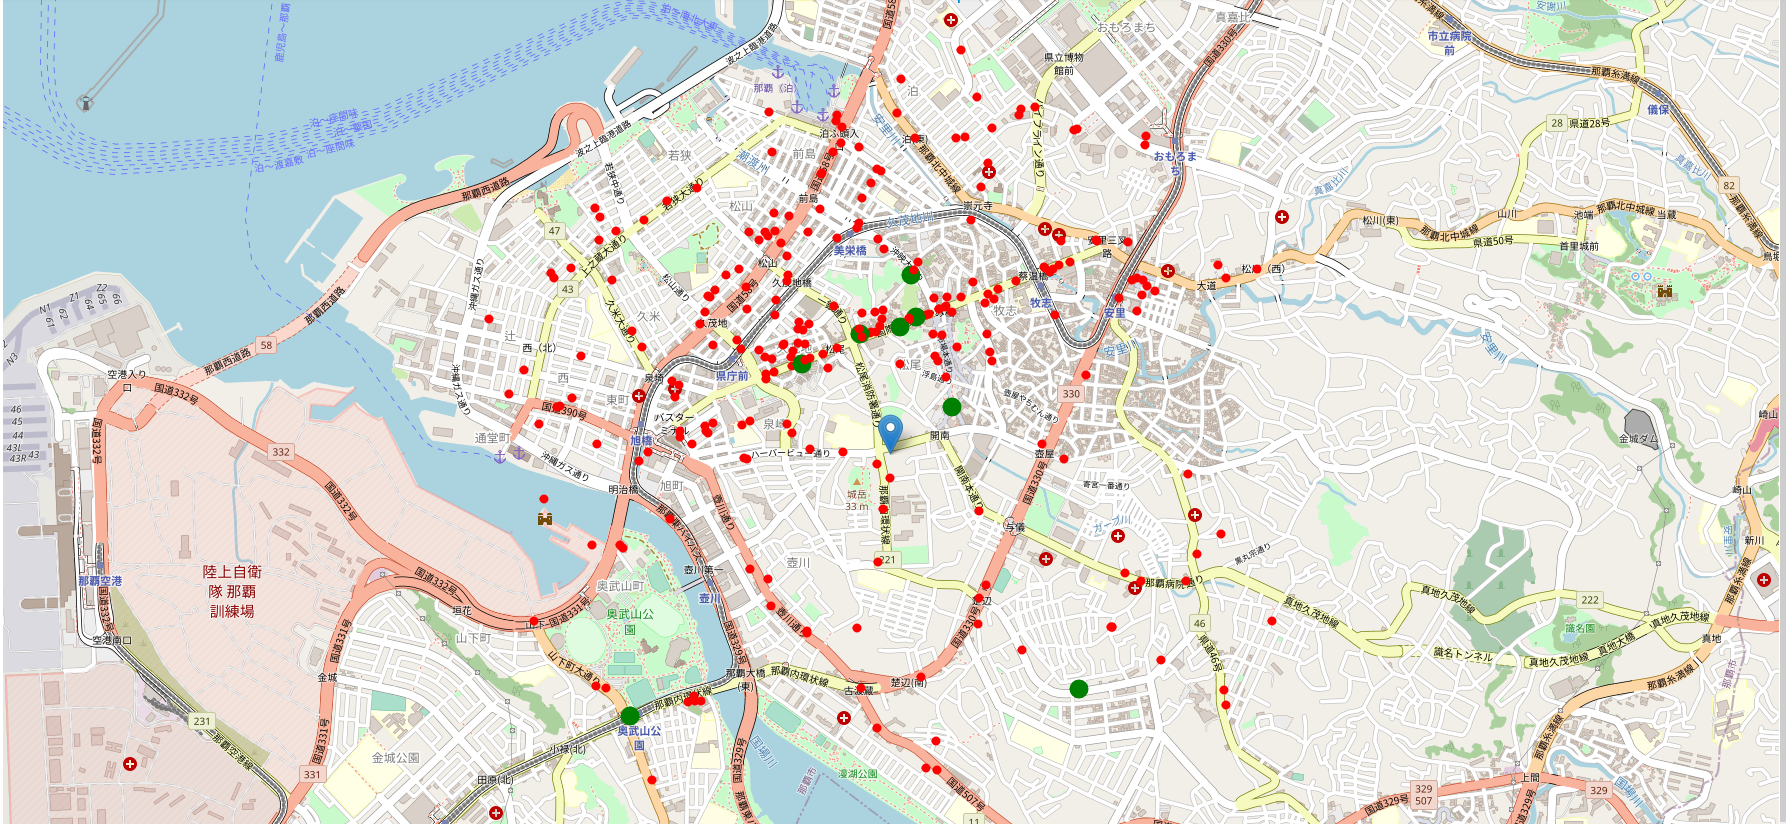
\includegraphics[scale=.3]{figures/cm2.png}
    \caption{Restaurants (red), Mexican Restaurants (green)}
    \label{fig:1}
\end{figure}

\subsection{Methodology}

In this project we will direct our efforts on detecting areas of Naha that have low restaurant density, particularly those with low number of Mexican restaurants. We will limit our analysis to area ~6km around city center.

In first step we have collected the required data: location and type (category) of every restaurant within 3km from IT College. We have also identified Mexican restaurants (according to Foursquare categorization).

Second step in our analysis will be calculation and exploration of 'restaurant density' across different areas of Naha - we will use heatmaps to identify a few promising areas close to center with low number of restaurants in general (and no Mexican restaurants in vicinity) and focus our attention on those areas.

In third and final step we will focus on most promising areas and within those create clusters of locations that meet some basic requirements established in discussion with stakeholders: we will take into consideration locations with no more than two restaurants in radius of 250 meters, and we want locations without Mexican restaurants in radius of 400 meters. We will present map of all such locations but also create clusters (using k-means clustering) of those locations to identify general zones / neighborhoods / addresses which should be a starting point for final 'street level' exploration and search for optimal venue location by stakeholders.


% --------------------
\section{Analysis}
% --------------------

Let's perform some basic explanatory data analysis and derive some additional info from our raw data. First let's count the number of restaurants in every area candidate:

\begin{figure}[H]
    \centering
        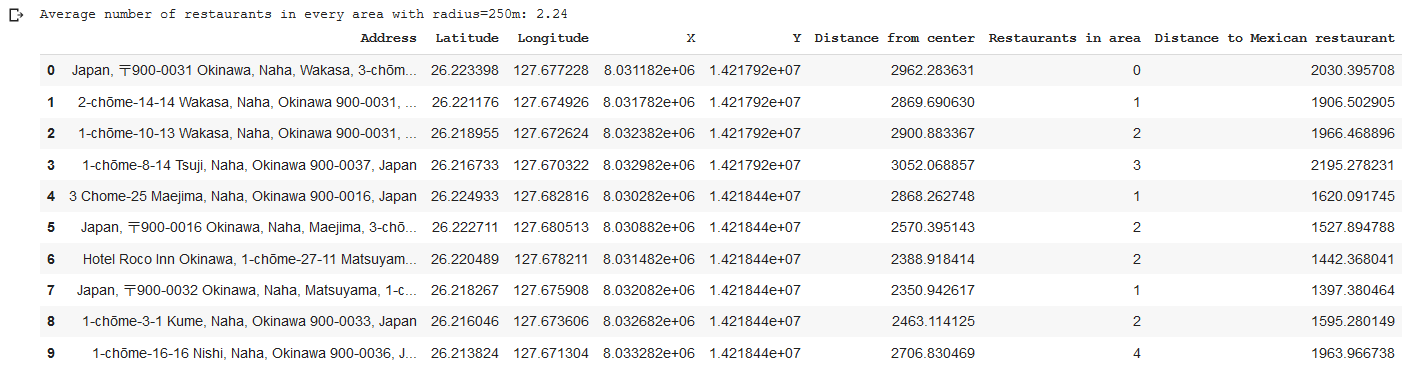
\includegraphics[scale=.4]{figures/cm3.png}
    \caption{Computed Restaurant distances.}
    \label{fig:1}
\end{figure}

Let's calculate the distance to Mexican restaurant from every area candidate center (not only those within 300m - we want distance to closest one, regardless of how distant it is).
(Go to Linked Jupyter Notebook for details)
On average Mexican restaurant can be found within ~1200m from every area center candidate.

Let's crete a map showing heatmap / density of restaurants and try to extract some meaningfull info from that.

\begin{figure}[H]
    \centering
        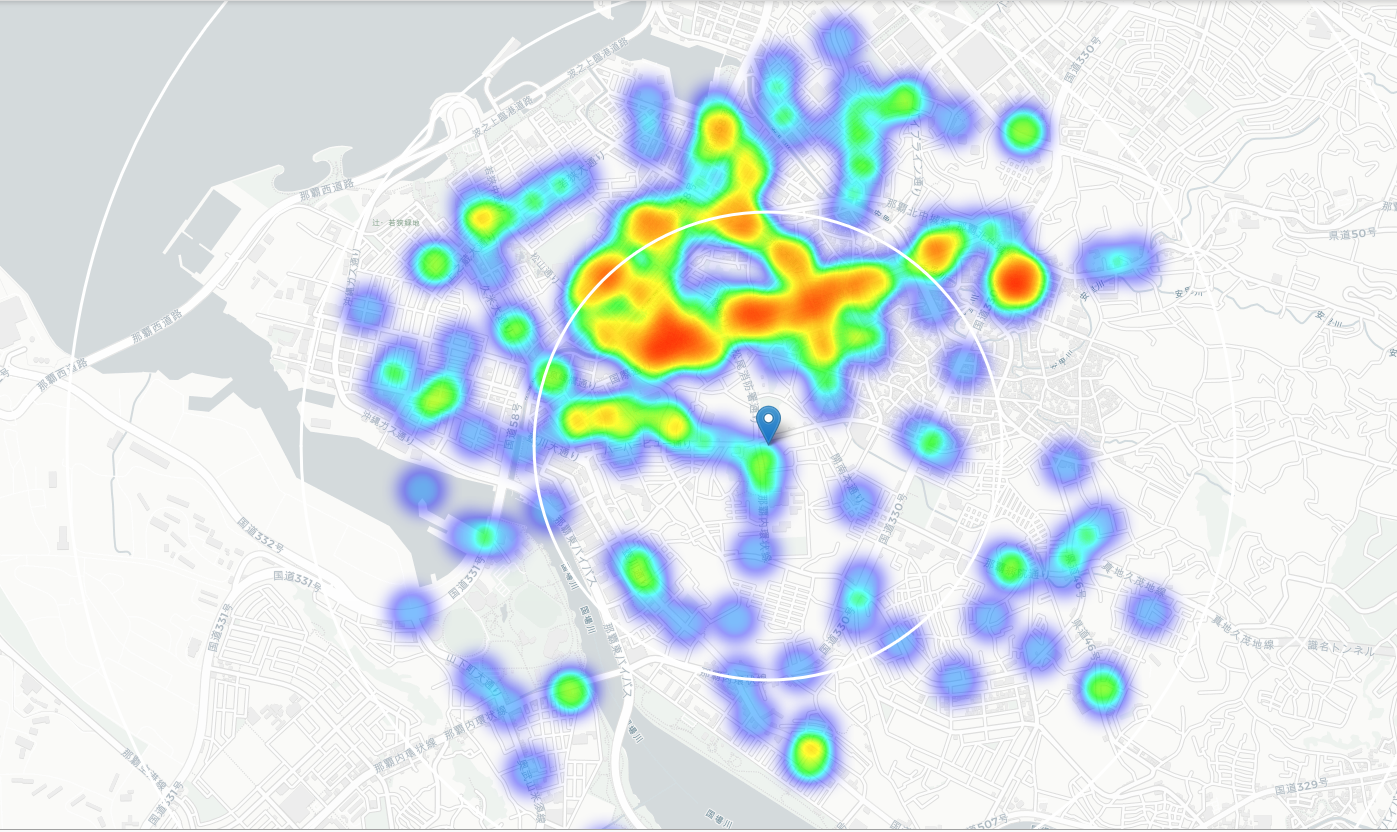
\includegraphics[scale=.4]{figures/cm4.png}
    \caption{Heatmap of Restaurants in the area.}
    \label{fig:1}
\end{figure}

Looks like a few pockets of low restaurant density closest to Naha center can be found south, south-east and east from IT College.

Let's create another heatmap map showing heatmap/density of Mexican restaurants only.

\begin{figure}[H]
    \centering
        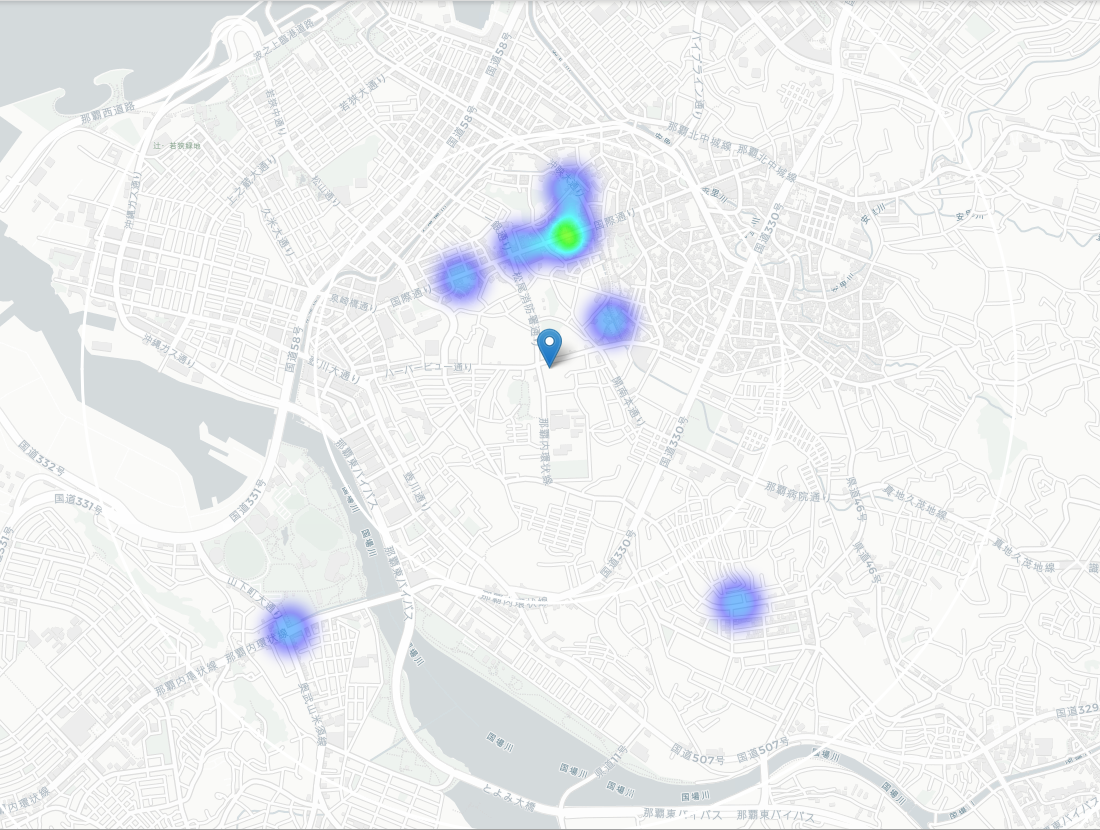
\includegraphics[scale=.4]{figures/cm5.png}
    \caption{Heatmap of Restaurants in the area.}
    \label{fig:1}
\end{figure}

This map is so 'cold' (Mexican restaurants represent a subset of ~8\% of all restaurants in Naha) but it also indicates higher density of existing restaurants directly north and west from IT College, with closest pockets of lowrestaurant density positioned east, south-east and south from city center.

Based on this we will now focus our analysis on areas south-west, south, south-east and east from IT College - we will move the center of our area of interest and reduce it's size to have a radius of 2.5km. This places our location candidates mostly in boroughs Asahimachi and Matsuo

\subsection{Asahimachi \& Matsuo}

Analysis with Google earth show Asahimachi and Matsuo as beautiful, interesting, highly populated and concurrent in the work hours.

This places also sport multiple recreation and shopping sites.

Asahimachi is just a bridge away from the Onoyama park and sports complex, also seems to have an activity boost for the nightlife thanks to some more turistic places nearby and a pachinko parlor inside the block.

Matsuo has a big park in it and offers many food places without being overcrowded with them like the surrounding areas, and most relevant a few blocks away you can finde the Naha Kokusai Dori Shopping Street.

Asahimachi

\begin{figure}[H]
    \centering
        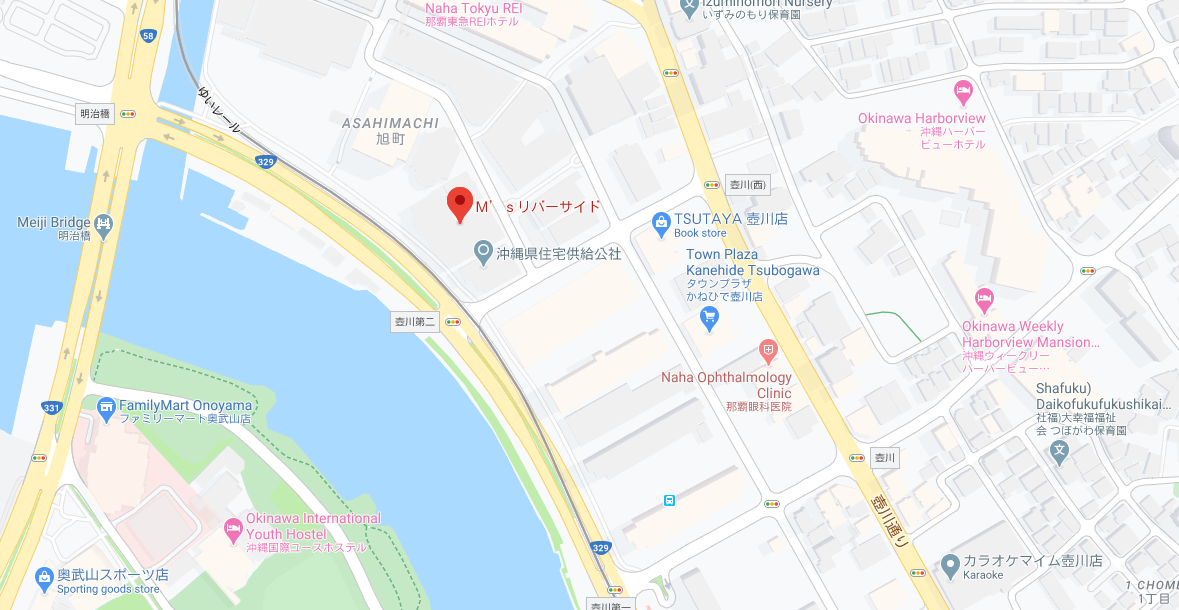
\includegraphics[scale=.4]{figures/asahimachi2.png}
    \caption{Asahimachi map view.}
    \label{fig:1}
\end{figure}

\begin{figure}[H]
    \centering
        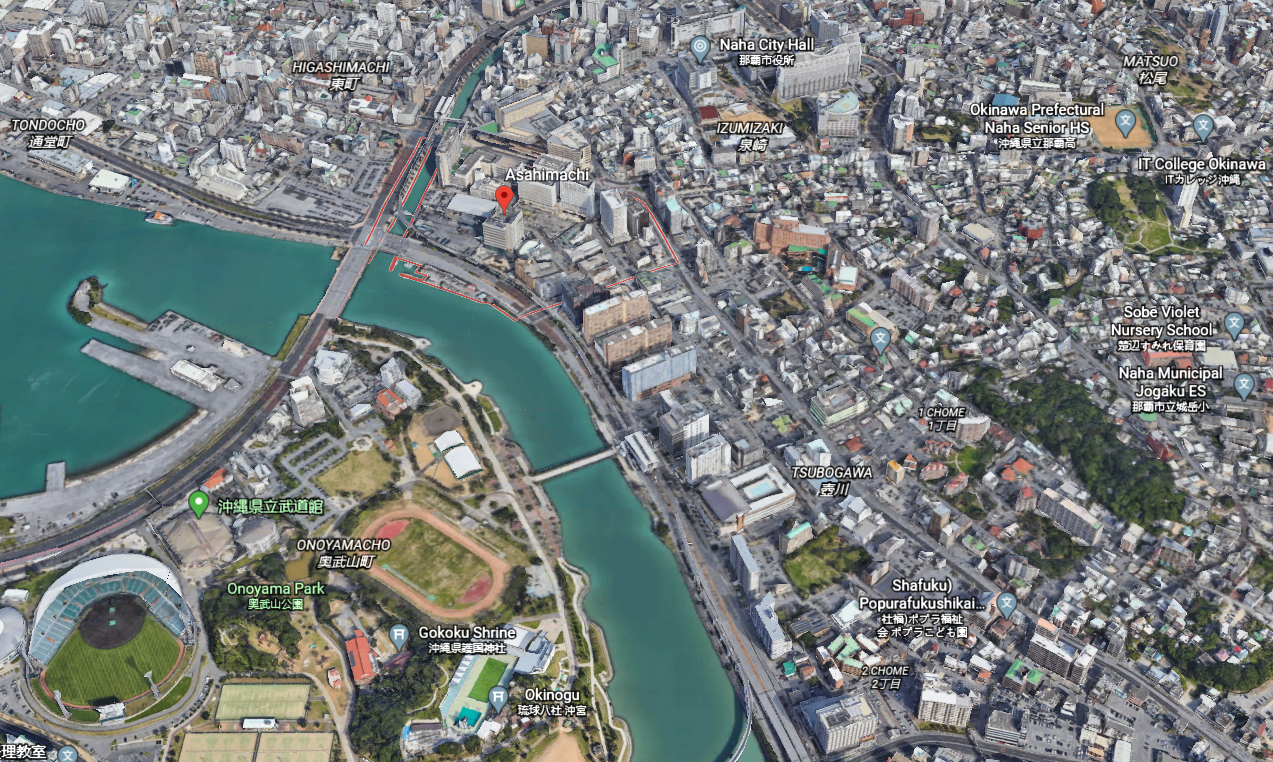
\includegraphics[scale=.4]{figures/asahimachi.png}
    \caption{Asahimachi satellite view.}
    \label{fig:1}
\end{figure}

\begin{figure}[H]
    \centering
        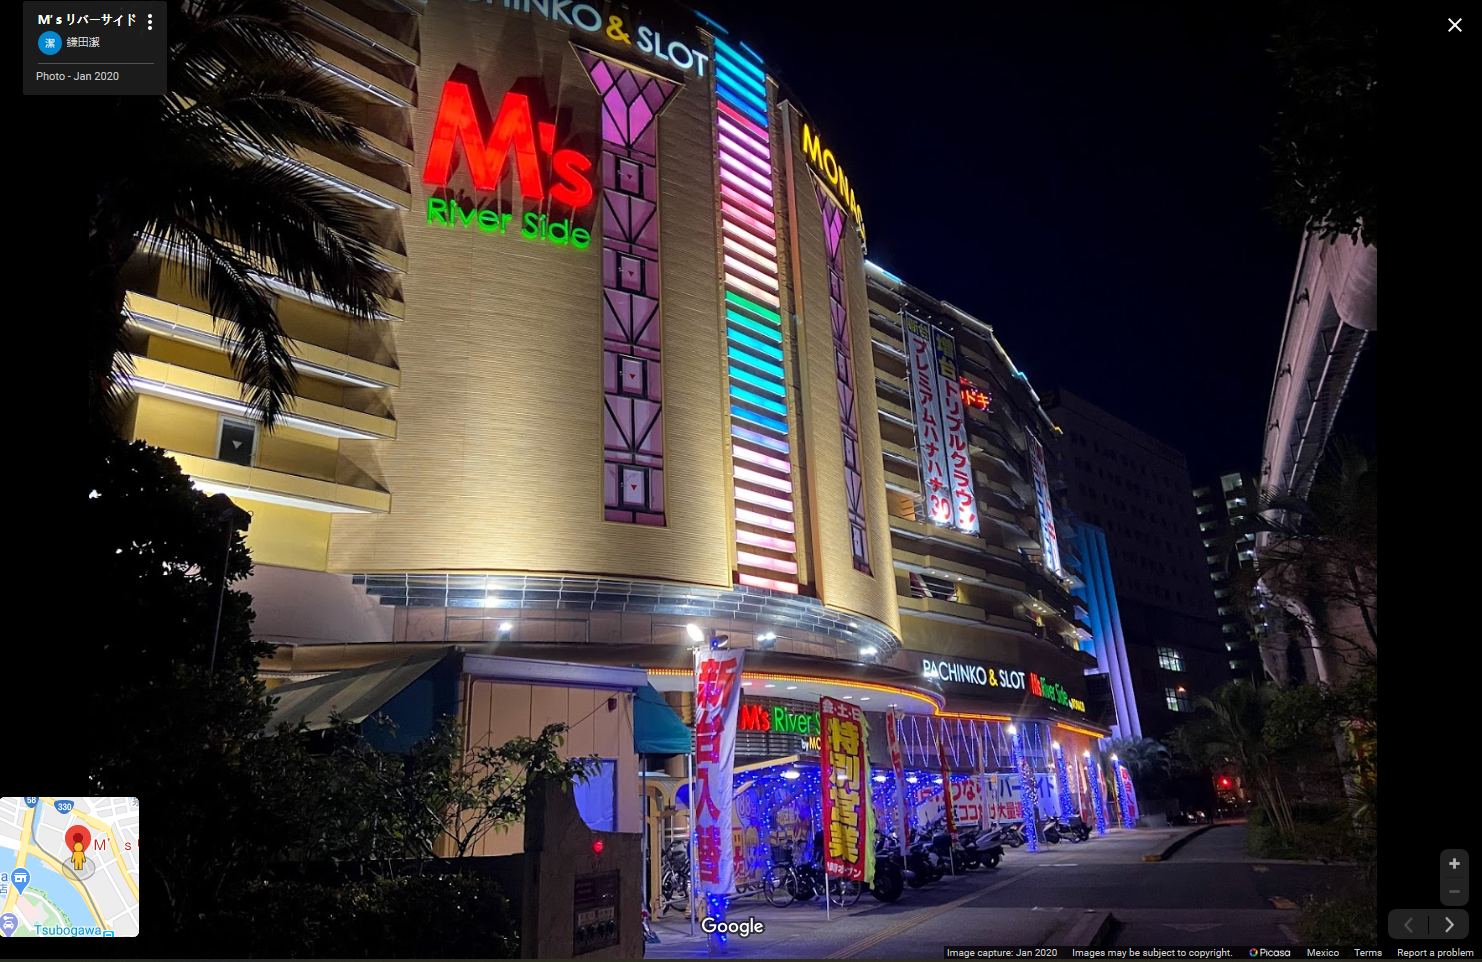
\includegraphics[scale=.4]{figures/asahimachi3.png}
    \caption{Asahimachi street view.}
    \label{fig:1}
\end{figure}

 Matsuo

\begin{figure}[H]
    \centering
        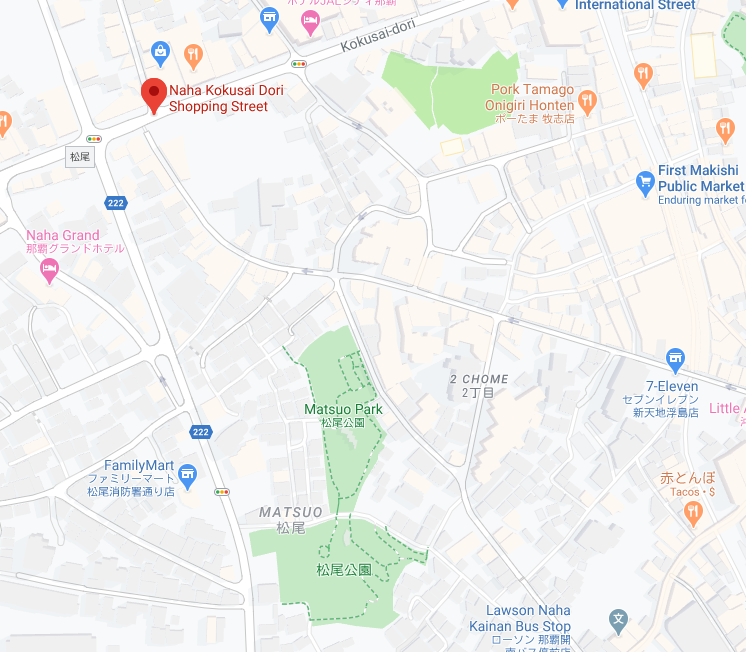
\includegraphics[scale=.4]{figures/matsuo2.png}
    \caption{Matsuo map view.}
    \label{fig:1}
\end{figure}

\begin{figure}[H]
    \centering
        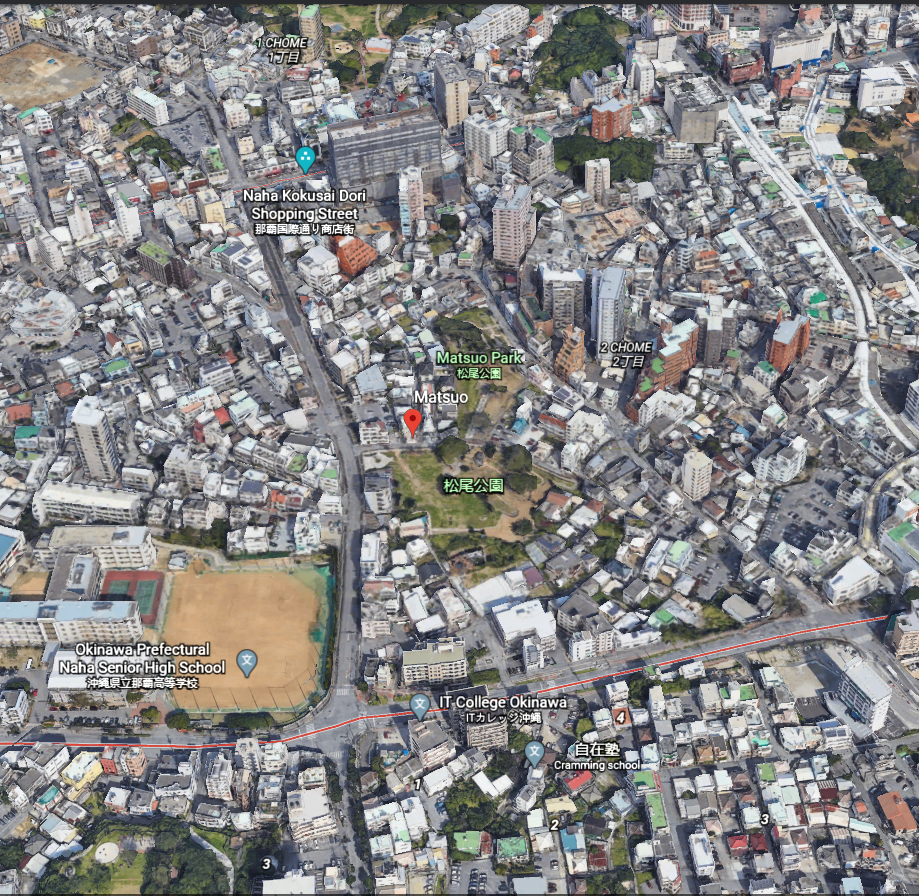
\includegraphics[scale=.4]{figures/matsuo.png}
    \caption{Matsuo satellite view.}
    \label{fig:1}
\end{figure}

\begin{figure}[H]
    \centering
        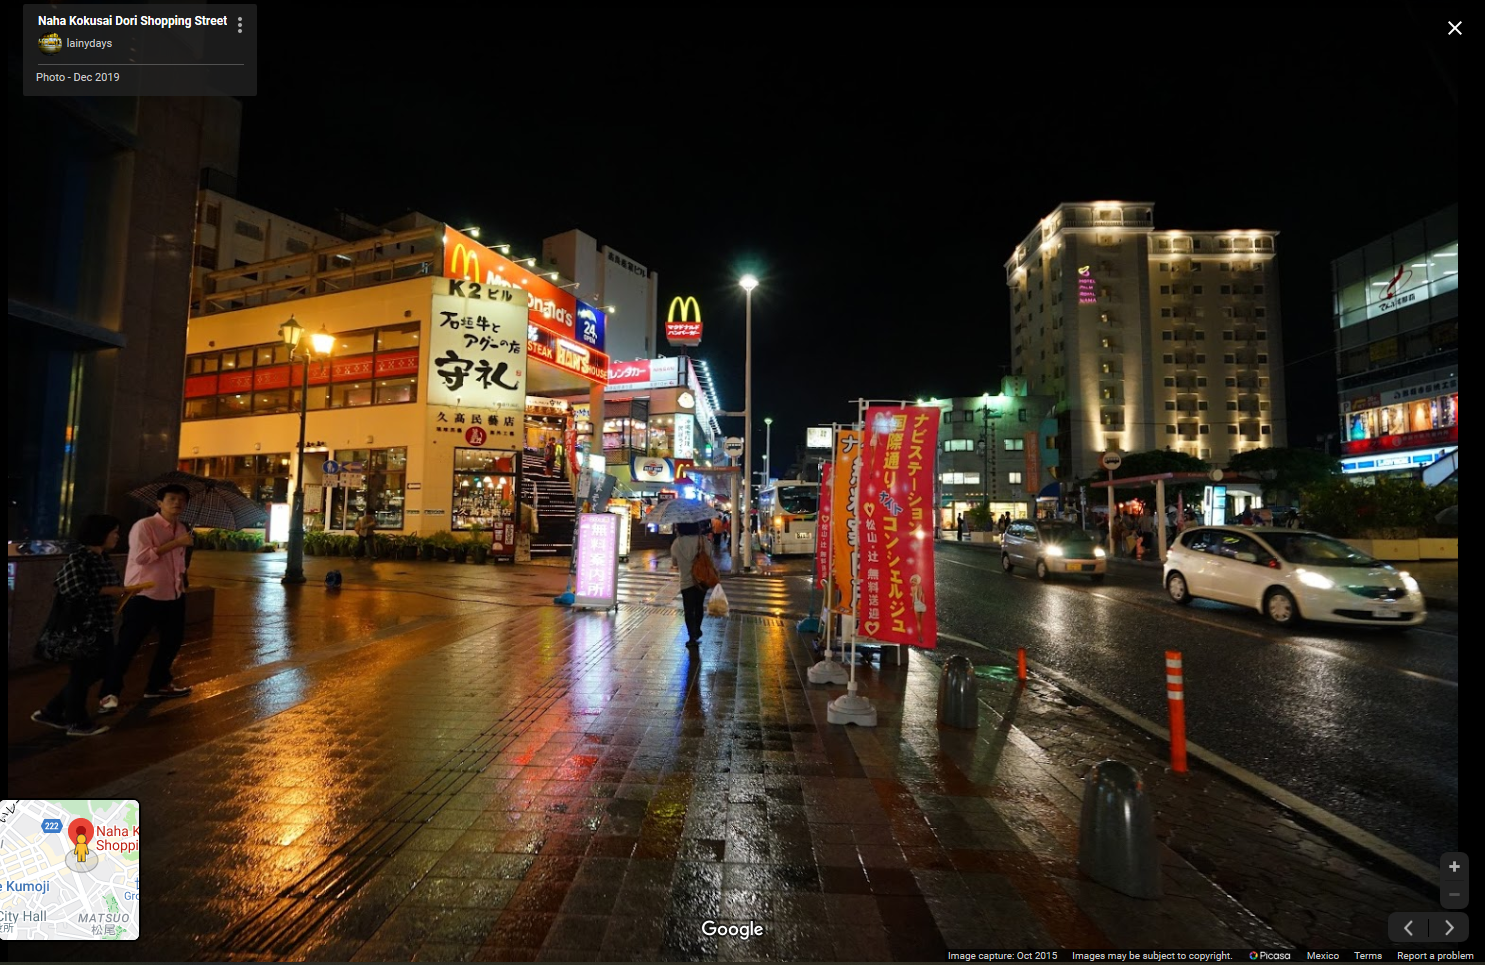
\includegraphics[scale=.4]{figures/matsuo3.png}
    \caption{Matsuo street view.}
    \label{fig:1}
\end{figure}


Let's also create new, more dense grid of location candidates restricted to our new region of interest (let's make our location candidates 170m appart), Now let's calculate two most important things for each location candidate: number of restaurants in vicinity (we'll use radius of 250 meters) and distance to closest Mexican restaurant.

\begin{figure}[H]
    \centering
        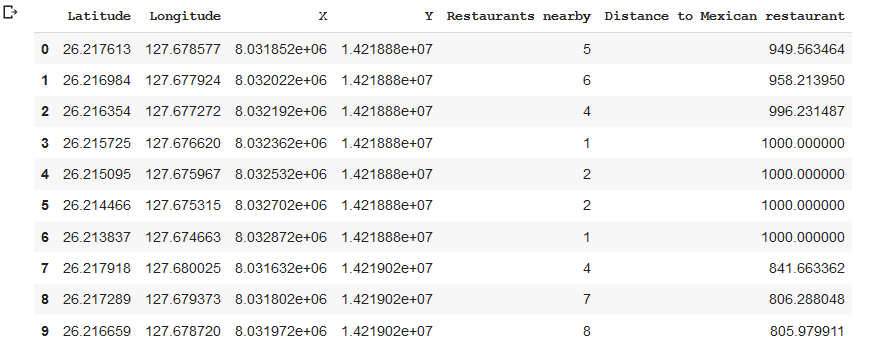
\includegraphics[scale=.8]{figures/cm7.png}
    \caption{Candidates.}
    \label{fig:1}
\end{figure}

It is Important to also  filter those locations: we're interested only in locations with no more than two restaurants in radius of 250 meters, and no Italian restaurants in radius of 400 meters.

\begin{figure}[H]
    \centering
        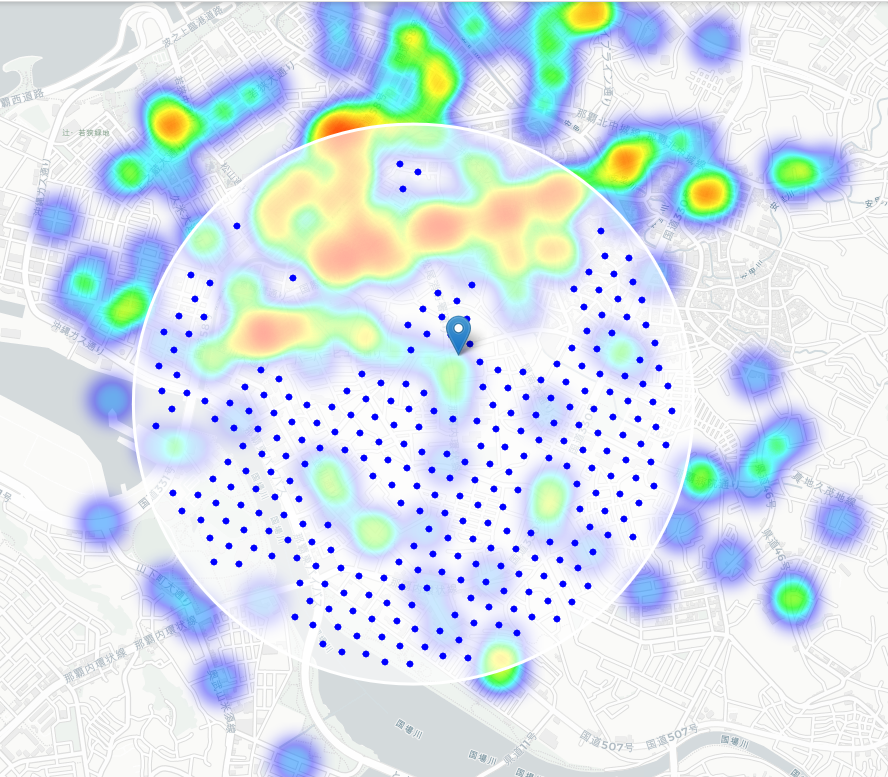
\includegraphics[scale=.4]{figures/cm8.png}
    \caption{Grid of candidate areas.}
    \label{fig:1}
\end{figure}


Now to test how well we are covering the interested ares lets make a union of the previous heat map with a new one for the proposed locations.

\begin{figure}[H]
    \centering
        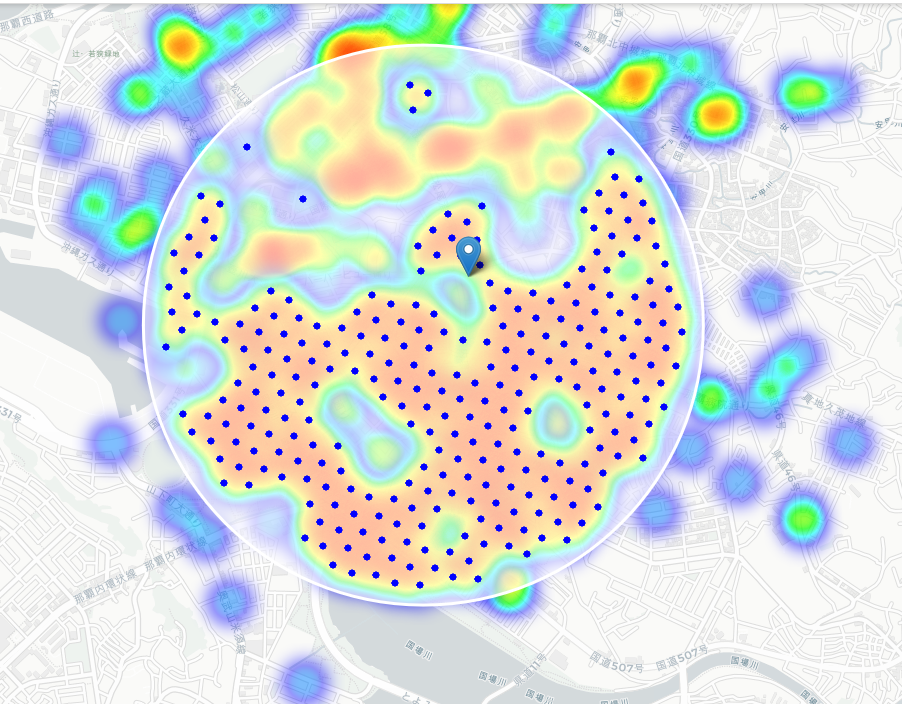
\includegraphics[scale=.4]{figures/cm9.png}
    \caption{ Union Heatmap current restaurant locations and candidate locations.}
    \label{fig:1}
\end{figure}

Let us now cluster those locations to create centers of zones containing good locations. Those zones, their centers and addresses will be the final result of our analysis. I decided to go for 50 clusters, thats a bit too much but, thats the best approximate number to cover the vast areas of interest, covering any point and avoid to much overlappin as well

\begin{figure}[H]
    \centering
        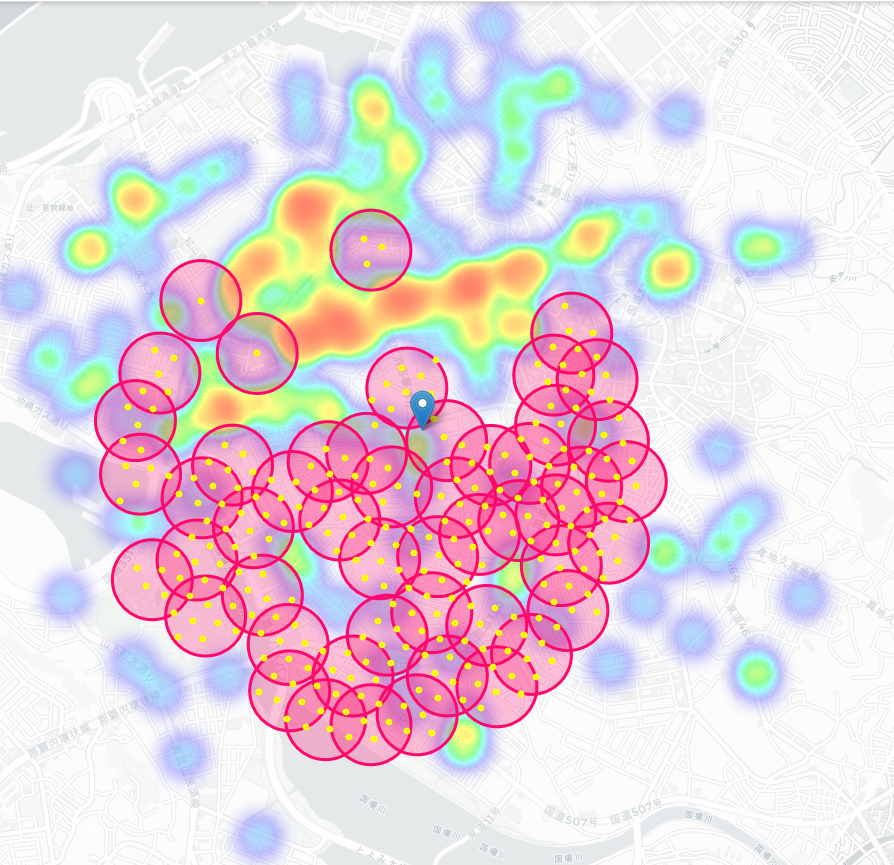
\includegraphics[scale=.4]{figures/cm10.png}
    \caption{ Clusters.}
    \label{fig:1}
\end{figure}

Not bad - our clusters represent groupings of most of the candidate locations and cluster centers are placed nicely in the middle of the zones 'rich' with location candidates.

Addresses of those cluster centers will be a good starting point for exploring the neighborhoods to find the best possible location based on neighborhood specifics.

Let's see those zones on a city map without heatmap, using shaded areas to indicate our clusters:

\begin{figure}[H]
    \centering
        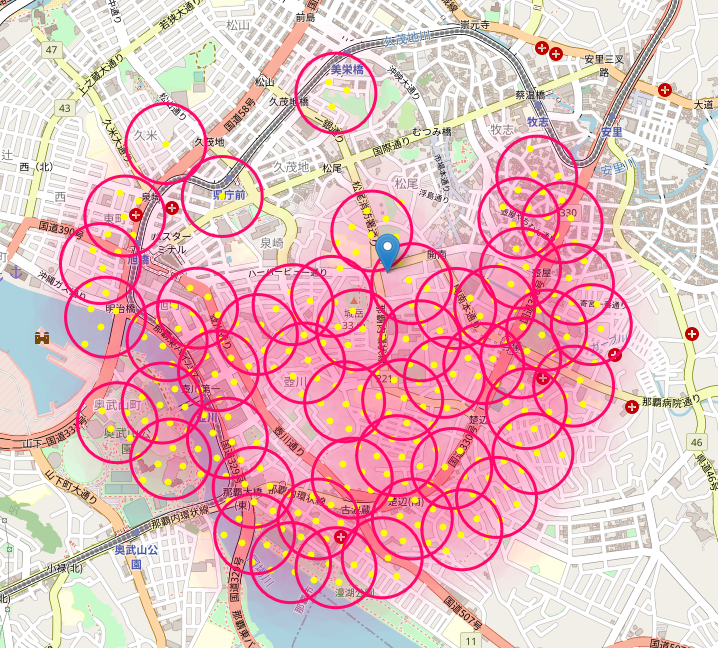
\includegraphics[scale=.4]{figures/cm11.png}
    \caption{ Shaded Clusters for better visibility.}
    \label{fig:1}
\end{figure}

\subsection{Asamichi and Matsuo clusters}

Let's zoom in on candidate areas near Asahimachi:

\begin{figure}[H]
    \centering
        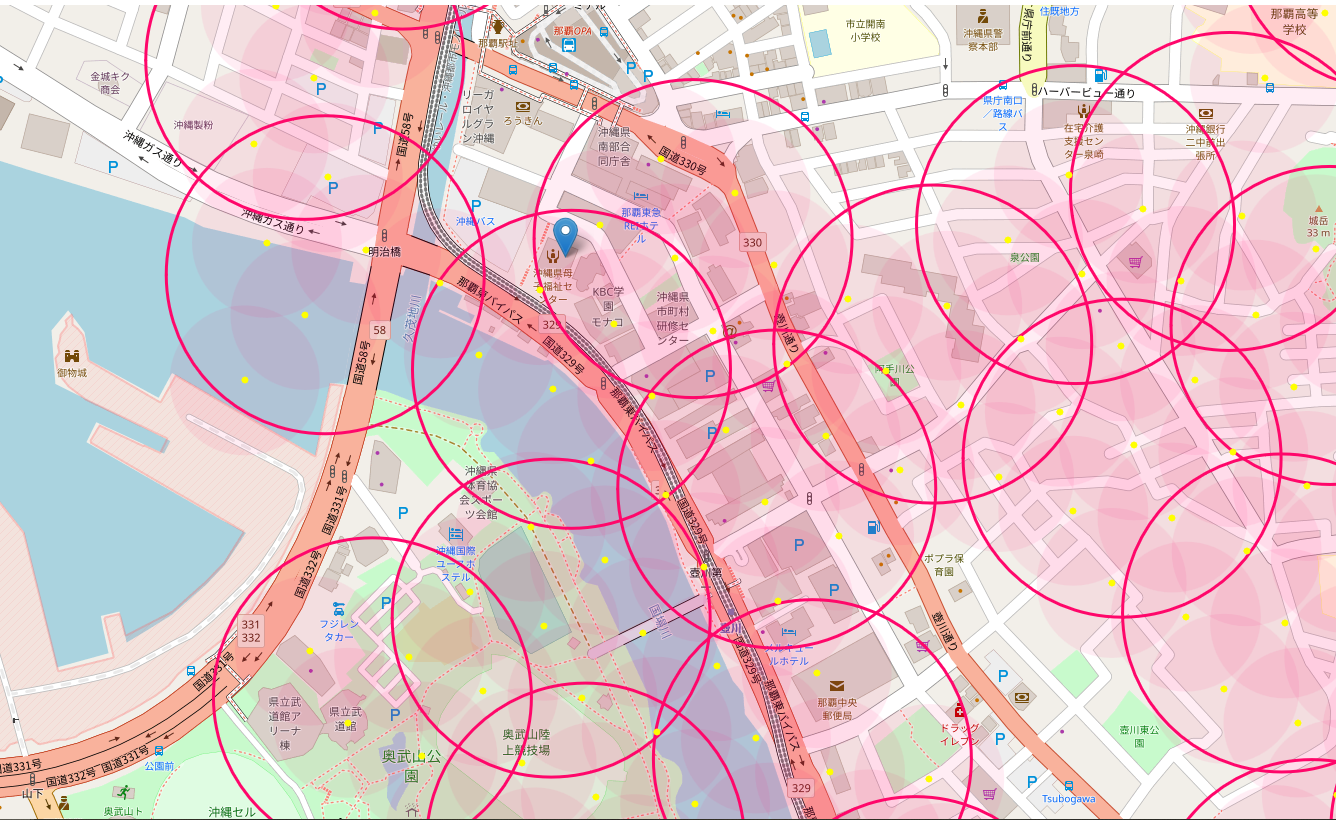
\includegraphics[scale=.4]{figures/cm12.png}
    \caption{ Viable locations near Asahimachi.}
    \label{fig:1}
\end{figure}


Let's zoom in on candidate areas near Matsuo:

\begin{figure}[H]
    \centering
        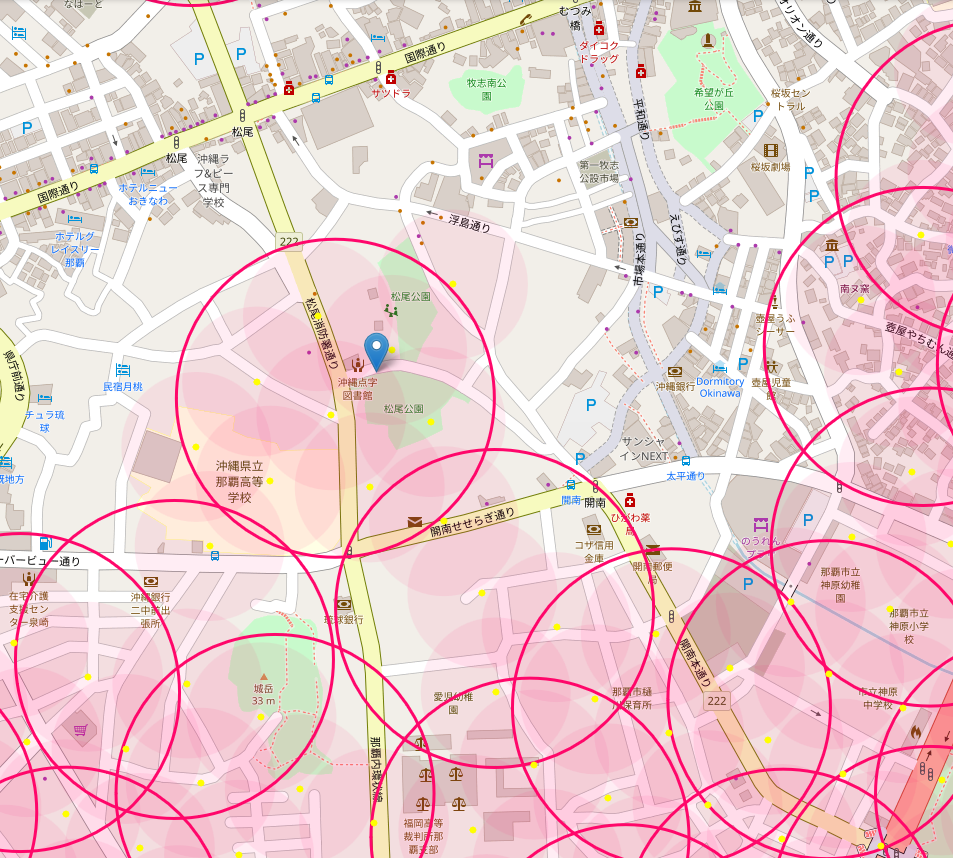
\includegraphics[scale=.4]{figures/cm14.png}
    \caption{ Viable locations near Matsuo.}
    \label{fig:1}
\end{figure}

\subsection{Final map with addresses}

Finaly, let's reverse geocode those candidate area centers to get the addresses which can be presented to stakeholders.

\begin{figure}[H]
    \centering
        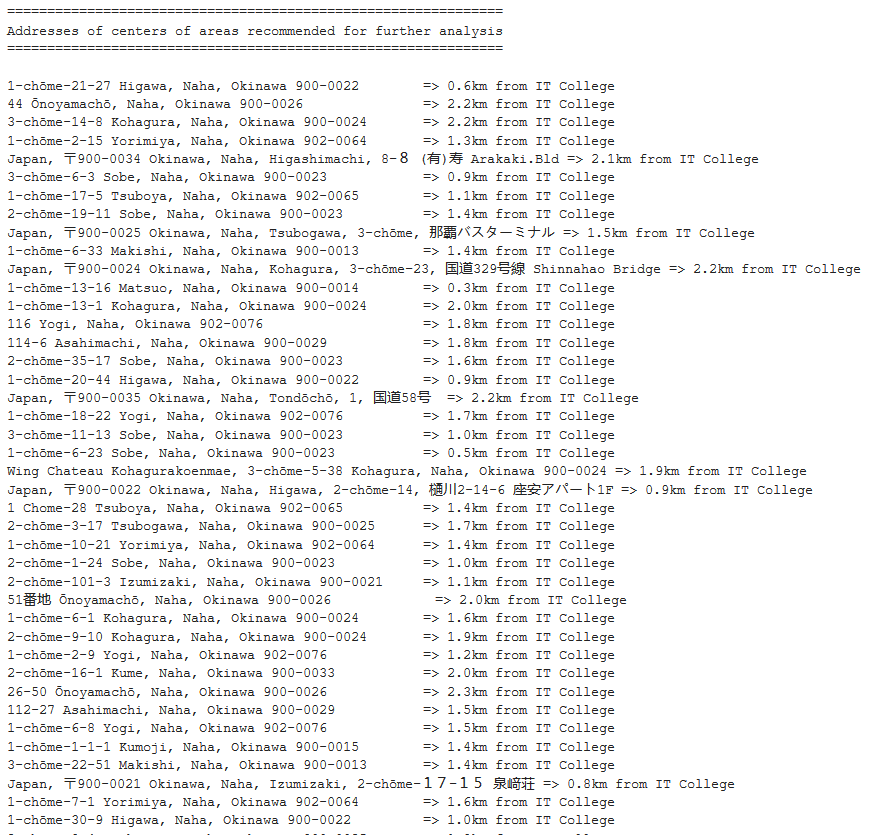
\includegraphics[scale=.6]{figures/cm16.png}
    \caption{ Found Addresses.}
    \label{fig:1}
\end{figure}

We have created 50 addresses representing centers of zones containing locations with low number of restaurants and no Mexican restaurants nearby, all zones being fairly close to city center (all less than 4km from IT College, and about half of those less than 2km from IT College). Although zones are shown on map with a radius of ~500 meters (pink circles), their shape is actually very irregular and their centers/addresses should be considered only as a starting point for exploring area neighborhoods in search for potential restaurant locations. 


\begin{figure}[H]
    \centering
        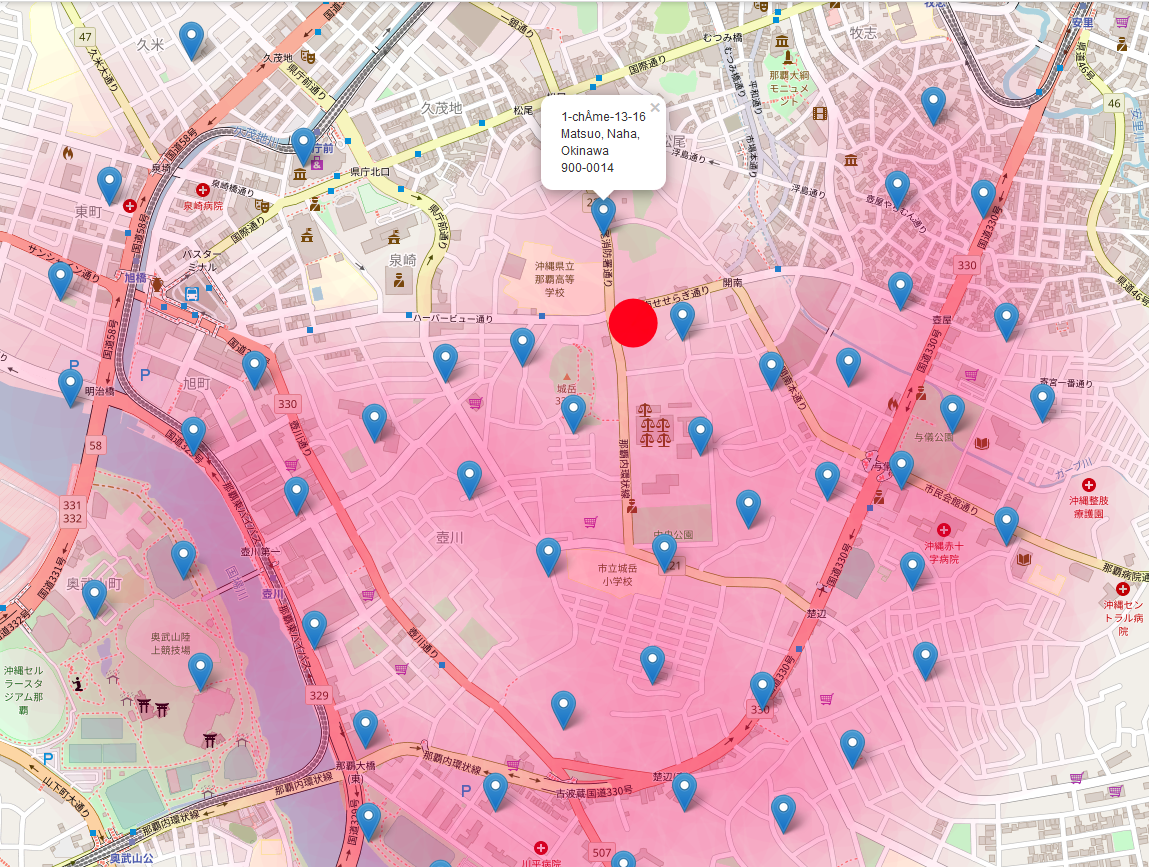
\includegraphics[scale=.5]{figures/cm15.png}
    \caption{ Viable addresses.}
    \label{fig:1}
\end{figure}

% --------------------
\section{Results and Discussion}

Our analysis shows that although there is a great number of restaurants in Naha (in our initial area of interest which was 6x6km around IT College), there are pockets of low restaurant density fairly close to city center. Highest concentration of restaurants was detected north and west from IT College. but our attention was focused on Adamaichi and Matsuo which offer a combination of popularity among tourists, closeness to city center, strong socio-economic dynamics and a number of pockets of low restaurant density.

After directing our attention to this more narrow area of interest (covering approx. 3x3km around from IT College) we first created a dense grid of location candidates (spaced 100m appart); those locations were then filtered so that those with more than two restaurants in radius of 250m and those with an Mexican restaurant closer than 400m were removed.

Those location candidates were then clustered to create zones of interest which contain greatest number of location candidates. Addresses of centers of those zones were also generated using reverse geocoding to be used as markers/starting points for more detailed local analysis based on other factors.

Result of all this is 50 zones containing largest number of potential new restaurant locations based on number of and distance to existing venues - both restaurants in general and Mexican restaurants particularly. This, of course, does not imply that those zones are actually optimal locations for a new restaurant! Purpose of this analysis was to only provide info on areas close to Berlin center but not crowded with existing restaurants (particularly Mexican) - it is entirely possible that there is a very good reason for small number of restaurants in any of those areas, reasons which would make them unsuitable for a new restaurant regardless of lack of competition in the area. Recommended zones should therefore be considered only as a starting point for more detailed analysis which could eventually result in location which has not only no nearby competition but also other factors taken into account and all other relevant conditions met.

\section{Conclusion}

Purpose of this project was to identify Naha areas close to center with low number of restaurants (particularly Mexican restaurants) in order to aid stakeholders in narrowing down the search for optimal location for a new Mexican restaurant. By calculating restaurant density distribution from Foursquare data we have first identified addresses that justify further analysis (Adamaichi and Matsuo), and then generated extensive collection of all other locations which satisfy some basic requirements regarding existing nearby restaurants. Clustering of those locations was then performed in order to create major zones of interest (containing greatest number of potential locations) and addresses of those zone centers were created to be used as starting points for final exploration by stakeholders.

Final decission on optimal restaurant location will be made by stakeholders based on specific characteristics of neighborhoods and locations in every recommended zone, taking into consideration additional factors like attractiveness of each location (proximity to park or water), levels of noise / proximity to major roads, real estate availability, prices, social and economic dynamics of every neighborhood etc.

More Data and Time is required.

\medskip
\bibliography{sample} 

\end{document}